\myChapter{Architectures}
\label{chap:Architectures}

In this chapter, an overview of the UNet and SRUNet model architectures used in the experiments is provided. Additionally, the employed training setup is outlined, which consists of a Generative Adversarial Network (GAN) framework that incorporates LPIPS and SSIM as the generator loss.

\section{UNet Architecture}
\label{sec:unet}

The UNet architecture was introduced by Ronneberger et al. \cite{ronneberger2015u} in 2015 for biomedical image segmentation tasks.

Let $x$ be a low-resolution input image with spatial dimensions of W x H x C, where W and H represent the width and height of the image, and C is the number of channels. The goal is to generate a high-resolution output image $y$ with spatial dimensions of W' x H' x C, where W' and H' are larger than W and H, respectively.

The UNet model is composed of an encoder and a decoder, with skip connections between them. The encoder takes the input image $x$ as input and applies a series of convolutional layers to reduce the dimensionality of the image and capture important features. The encoder can be represented as a function $f_\theta$ that takes the input image $x$ and returns a feature map \textbf{f}:

$$ \textbf{f} = f_\theta(x) $$

The decoder takes the feature map \textbf{f} as input and applies a series of convolutional layers to upsample the image while preserving the details. The decoder can be represented as a function $g_\phi$ that takes the feature map \textbf{f} and returns the generated high-resolution output image $\hat{y}$:

$$ \hat{y} = g_\phi(\textbf{f}) $$

The skip connections are used to connect the corresponding encoder and decoder layers. Specifically, the feature maps from the encoder are concatenated with the feature maps from the corresponding decoder layers to help the model capture the fine-grained details and ensure that the output image is accurate.

$$ z = x + W_2\sigma(W_1 x + b_1) + b_2 $$

where $W_1$ and $W_2$ are weight matrices, $b_1$ and $b_2$ are bias vectors, and $\sigma$ is a non-linear activation function.

\Cref{fig:unet} shows a high-level representation of the UNet architecture.

\begin{figure}[ht]
\centering
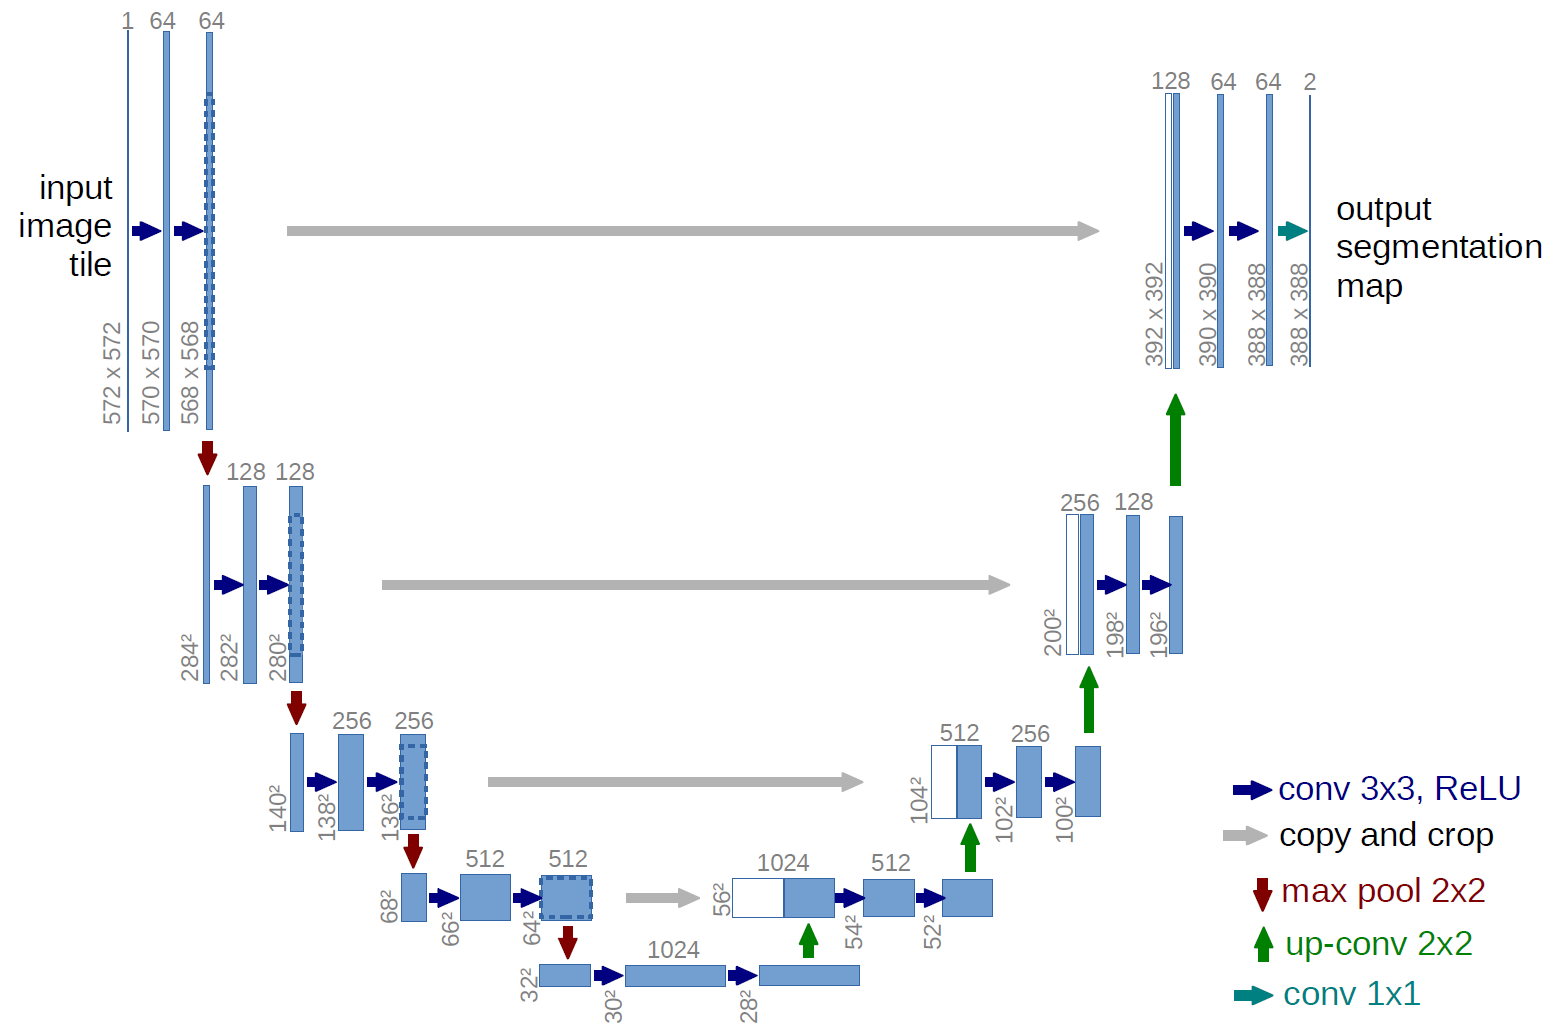
\includegraphics[width=1.0\textwidth]{static/unet_architecture.png}
\caption{UNet architecture. The name is inspired by its shape like a U. It has a contracting path on the left side, a fully-connected layer in the middle, and an expansive path on the right side. The contracting path consists of repeated blocks of convolutional layers followed by ReLU activation and ending with max-pooling. The output is passed through a fully-connected layer and then to the expansive path. The expansive path has the same number of blocks as the contracting path but up-samples instead of max-pooling. The input to each block is the output of the previous block concatenated with the corresponding block from the contracting path.}
\label{fig:unet}
\end{figure}

\section{SRUNet Architecture}
\label{sec:srunet}

SRUNet is an adaptation of the UNet architecture for super-resolution and compression artefact removal, proposed in \cite{vaccaro2021fast} by Vaccaro et al. The main two modifications are the decrease in the number of filters in each convolutional layer, and the use of a residual layer as the final layer.

The final residual layer computes the difference between the input image $x$ scaled up with a linear interpolation function and the output of the second to the last layer scaled up with the pixel shuffle function. In this way, the model is set to learn the difference between a low-resolution image and its high-resolution version.

Pixel-shuffle (also known as sub-pixel convolutional layer), is the fastest up-sample layer available: it comprises a depth-compression of the output tensor into 12-channels via convolution operation, and then these features are reshuffled into an RGB image but at double resolution. Alternatives, such as bilinear upsample with convolution, the transposed convolution, or even the reshuffling to a higher dimension with the same depth, would add an exaggerated overhead since they would work in the high-resolution space.

Modelling the problem as producing a residual on the top of the up-sampled image is particularly convenient. This forces the model to focus on the high-frequency patterns sharpening edges or increasing texture details since the low-frequency patterns are still from the up-sampled image. Furthermore, faster convergence of the training process is ensured.
 
\Cref{fig:srunet} shows a high-level representation of the SRUNet architecture.

\begin{figure}[ht]
\centering
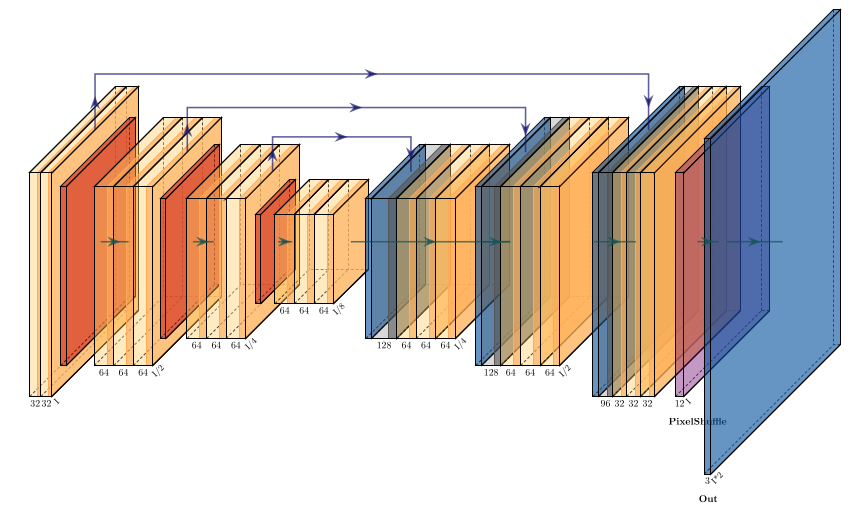
\includegraphics[width=1.0\textwidth]{static/srunet_architecture.png}
\caption{SRUNet architecture. It differs from a classical UNet architecture mainly by the decrease in the number of filters in each convolutional layer, and the use of a residual layer as the final layer.}
\label{fig:srunet}
\end{figure}

\section{Training Setup}
\label{sec:training-setup}

To train both the UNet and SRUNet models, a Generative Adversarial Network (GAN) framework was employed. Introduced in \cite{goodfellow2020generative}, the GAN framework consists of two models, a generator and a discriminator.

In the context of super-resolution, the generator network takes a low-resolution image as input and generates a high-resolution image, while the discriminator tries to distinguish between the generated high-resolution image and the true high-resolution image.

The two networks are trained in an adversarial manner: the generator tries to fool the discriminator by generating high-resolution images as similar as possible to the ground-truth images, while the discriminator tries to correctly classify the generated images as true or generated. This competition between the two networks leads to the generator improving over time and producing images with more quality.

The generator loss is composed of two parts: an adversarial loss and a content loss.
The generator is encouraged to generate high-resolution images that appear as much as possible to come from the distribution of the ground-truth images by the adversarial loss and to generate high-resolution images that are as close as possible to the actual ground-truth images by the content loss.

In this setup, LPIPS and SSIM were used as the content loss. LPIPS is a perceptual similarity metric that measures the distance between two images in terms of their perceptual features. SSIM is a structural similarity metric that measures the similarity between two images in terms of their structure, luminance, and contrast. See \cref{chap:Metrics}, for further details on perceptual and non-perceptual metrics. 

The generator loss can be represented as follows:

$$
    \mathcal{L}_{G} = \underset{
        \text{adversarial loss}
    }{\underbrace{
        -\log(D(\hat{y}))
    }} + \underset{
        \text{content loss}
    }{\underbrace{
        w_{LPIPS}\cdot LPIPS(\hat{y}, y) + w_{SSIM} \cdot (1 - SSIM(\hat{y}, y))
    }}
$$

where $\hat{y}$ is the generated high-resolution image, $y$ is the ground truth high-resolution image, $D(\hat{y})$ is the probability score outputted by the discriminator for the generated image, $w_{LPIPS}$ and $w_{SSIM}$ are hyperparameters that control the relative importance of the LPIPS and SSIM losses.

The design chosen for the discriminator network is the same as the one used in \cite{ledig2017photo}, where the authors followed the architectural guidelines described in \cite{radford2015unsupervised} and incorporated LeakyReLU \cite{maas2013rectifier} activation with $\alpha$ set to 0.2 (see \cref{fig:leakyrelu}) while avoiding max-pooling in the network.

\begin{wrapfigure}{r}{0.4\textwidth}
\centering
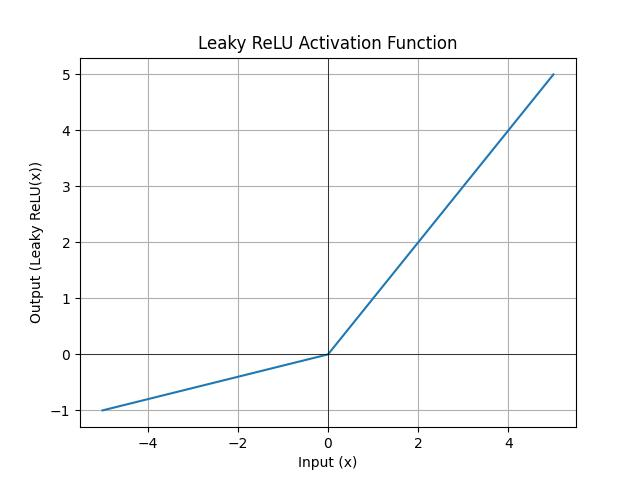
\includegraphics[width=0.4\textwidth]{static/LeakyReLU.jpg}
\caption{LeakyReLU ($\alpha$ := 0.2).}
\label{fig:leakyrelu}
\end{wrapfigure}

The discriminator network structure is illustrated in \cref{fig:discriminator}. It includes eight convolutional layers, with a 3$\times$3 filter kernel size that increases by a factor of 2, ranging from 64 to 512 kernels, similar to the VGG network \cite{simonyan2014very}. Strided convolutions are employed to decrease the image resolution each time the number of features doubles. The final output of 512 feature maps is fed into two dense layers, followed by a sigmoid activation function to obtain a classification probability for the input sample.

\begin{figure}[ht]
\centering
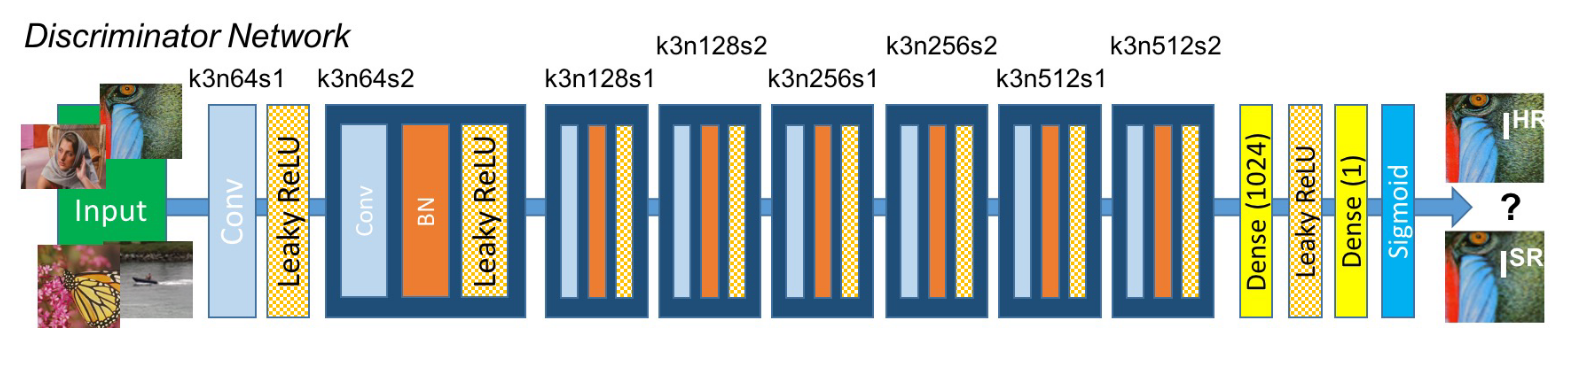
\includegraphics[width=1.0\textwidth]{static/discriminator_architecture.png}
\caption{The architecture of the discriminator network with corresponding kernel size (k), number of feature maps (n) and stride (s) indicated for each convolutional layer.}
\label{fig:discriminator}
\end{figure}

During the model training process, the Adam optimizer was utilized with a learning rate of $1\times10^{-4}$. The model was trained for 191,268 iterations, with each batch consisting of 14 image patches randomly sampled from the training set. A patch size of 96$\times$96 was used, with one random crop per image. The sole data augmentation strategy applied was the horizontal reflection, avoiding warping or rotation transforms to maintain consistency with real H.265-encoded frames.

Model training required approximately 72 hours on a single NVIDIA Titan Xp. The proposed model was trained using the BVI-DVC dataset \cite{ma2021bvi}, designed for deep video compression tasks. This dataset includes 200 frame sequences truncated at the 64\textsuperscript{th} frame, with frame rates ranging from 25 to 120. The sequences feature various content types, such as natural scenes, man-made objects, and cityscapes, with some examples shown in \cref{fig:bvi-dvc}.

\begin{figure}[ht]
\centering
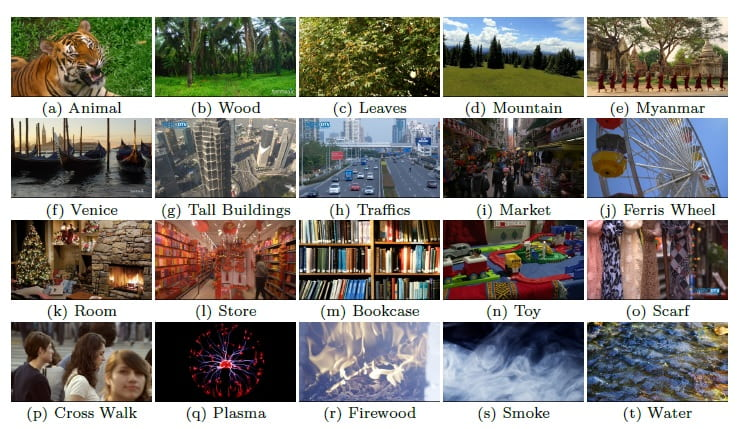
\includegraphics[width=1.0\textwidth]{static/BVI-DVC.jpg}
\caption{Some frame examples from the BVI-DVC dataset.}
\label{fig:bvi-dvc}
\end{figure}

While the original resolution was 2160p, the dataset authors created down-scaled versions at 1080p, 540p, and 270p, yielding 800 sequences and a total of 51,200 frames. The original BVI-DVC dataset served as the ground truth for the training dataset. Input data was generated by compressing each sequence using the H.265 codec with a Constant Rate Factor (CRF) of 23 while reducing the resolution to one-quarter of the original size. Fixing the CRF aimed to mitigate the mode-collapse issue described in \cite{galteri2019deep}. However, it should be noted that a fixed CRF does not guarantee uniform frame quality; for example, frames with motion might exhibit lower quality than stationary ones.

Training the models on compressed videos, rather than only the down-scaled version of high-quality videos, was crucial for applying super-resolution to compressed videos and performing both artefact reduction and super-resolution. Training the model solely for super-resolution could result in the model failing to detect features to super-resolve or even enlarging compression artefacts and reducing overall quality.
